\documentclass[12pt,notitlepage,oneside]{report}
\setcounter{secnumdepth}{3}
\usepackage{buet_msc_thesis}
\usepackage{lipsum}
\usepackage{sectsty}
\chapternumberfont{\fontsize{17}{15}\selectfont}
\chaptertitlefont{\fontsize{17}{15}\selectfont}
\sectionfont{\fontsize{14}{15}\selectfont}
\subsectionfont{\fontsize{12}{15}\selectfont}
%\usepackage[acronym, toc]{glossaries}

% Uncomment any of the following lines should you need to
% suppress the LOF, or LOT or LOA

% \suppresslistoffigures 
% \suppresslistoftables
% \suppresslistofalgorithms

% For index creation, comment this out if you do not want to create an
% index
\makeindex[intoc]
\patchcmd{\titlepage}{empty}{fancy}{}{}
\patchcmd{\chapter}{plain}{fancy}{}{}
\begin{document}


% Edit as needed below this line
% %%%%%%%%%%%%%%%%%%%%%%%%%%%%%%%%%%%%%%%%%%%%%%%%%%%%%%%%
% Chapter-1

\chapter{Introduction}\label{intro}
 At present there are millions of sites, applications, blogs that deal with text data. Most of the data deals with complex emotions of the people. Sometimes it is about a bad product, sometimes it is simply about someone's mental health condition. In order to sort all the data and make sense of it, a system is necessary.And it is not possible for a human being to make sense of millions and billions of data. So different language processing methods was created. Methods that can give results after processing thousands of data. These methods include models like RNN, LSTM, NLP.

Long short term memory or for short, LSTM is type of recurrent neural network. It is more like a modified version which can easily remember past data in memory. LSTM uses back propagation to train itself. So the solution we discuss is to implement LSTM to detect emotions more accurately from texts using better computation methods. 

\section{Problem Statement}
The problem is that we have huge data and not enough ways to process it and get a intended outcome. Existing models don't always give accurate results on the emotion the textual data is expressing. It can easily be identified by a human but it needs to be done by machines or simply computers more efficiently using less resources while computing the result. Because a lot of the existing methods rely on heavy computational resources. By using LSTM and modifying to give better output. 

We implement emotion detection and train it with datasets from kaggle which contains data consisting of mainly four emotions. Deep learning methods has been utilised for sentence analysis and processing of emotional data. Various approaches exist today for detecting emotion from text but often it is only limited to three categories, positive, negative and neutral. Deep learning technique provides the ability to classify different emotions as well from text data.
\section{Problem Background}
Neural networks plays an important role in the world of deep learning. There are a lot of neural network models which are used for this purpose. But ass discussed earlier, not all of them provides efficient results. For example, CNN can also be used to identify emotions from texts but it has a drawback, it doesn't store the trained knowledge for it to be used later. The network needs to be trained every time we want to run tests. It starts from scratch again. That's why older neural network models cant utilize the benefit of memory storage. That's why we have deep learning capable algorithms such as LSTM, BI-LSTM which learns each and every word from the given sentences present in the corpus.   

\section{Motivations}

We are currently seeing a boom in social media popularity and ecommerce sites. More than half of the world uses social media for different interactions and a quarter of the people now prefer ecommerce sites for purchases of different necessities. The use of texts in these sites is seen excessively as people share their opinions as posts, blogs and reviews in social media and reviews of products in different ecommerce sites. As a result, we now have a very big resource in our hand which can be used for providing tailor made services for the customers by service providers. Determining emotion from texts can help us reach a verdict on a topic or a product from thousands or millions of people. It will be possible to determine whether a service is appreciated or hated by the people simply from their posts, reviews in an instant, saving tons of time and playing a big role in product improvement. Furthermore, it can be also applied in applications such as emotion retrieval from suicide notes, detecting insulting sentences in chat conversations and so on. Therefore, a better method of detecting emotion from text based data is very crucial in the modern world.

\section{Research Objectives}
There are many emotion detection techniques but not all of them provide state of
the art accuracy. There are abundant ways to make it more efficient and less time
consuming on the hardware capability end. The objectives of this project include –
\begin{itemize}
\item To better understand the concept of LSTM model and its word embedding techniques
\item To improve accuracy of emotion detection from texts using LSTM model
\item To detect wide range of emotions from given text in terms of anger, fear, joy and sadness 
\item To build a better algorithm to be implemented in applications like sentiment analysis
\end{itemize}

\section{Significance of the Research} 
Emotion detection allows the ability to extract insights from comments on social media, survey data or other sources of feedback methods. These insights are often helpful in understanding targeted people's perspective. It can also be used to determine mental condition of suicidal patients from their diaries or blogs. Which is why emotion detection is greatly important in this digital era. Therefore accurate results from such research will be of great importance to the world. 

\section{Key Contribution}
This research offers its contribution in improving accuracy of LSTM by fine tuning its architecture, improving performance with data training and optimizing it to have better learning rate and proper weight initialization.

% Chapter-2
\chapter{Background Study} \label{ch:literature_review}


Emotions that incite individuals to write down certain words at particular times are what emotion detection is about. People often convey their feelings through texts, words. That's why it has been the topic of research for many. Researchers often try to create or innovate or perfect systems to better understand how emotions can be extracted in a meaningful way. Deep learning has also paved the way for researchers to further study this topic.
\section{Literature Review}

\subsection{Emotion Correlation Mining Through Deep Learning Models on Natural Language Text}
Xinzhi Wang et al.[1] introduced an embedded recursive neural network for improving emotion recognition, Long Short-Term Memory (LSTM) was used as a variant of RNNs. This method determines to do the potential and meaningful correlation among emotions from Web news. Tow deep neural network models, CNN-LSTM2 and CNN-LSTM-STACK are employed for emotion recognition. The data sets are collected from one of the most popular social platforms, news channel. Emotion correlation differs for different types datasets. In objective texts, some emotions be misinterpreted as love. Also, emotions are easily mistaken as anger. Yet, it achieved greater than 85\% and approaches 90\%.


\subsection{Topic-Enhanced Capsule Network for Multi-Label Emotion Classification}
Donghong Ji et al.[2] developed a capsule network which is effectively leveraging for multiple emotion prediction. This model consists of two components, a topic module and a capsule model. The topic module takes Bag of Words (BoW) as input via Variational Autoencoder (VAE) and learns latent topics and keywords. Then the capsule module captures encapsulated features for each emotion from low level to high level via three deep capsule layers. In the learning process, they pre-train the emotion module and co-train the entire part with a batch size of 16, both under early-stop strategy. Results on the benchmark data-sets showed that their method outperformed strong baselines by a large margin.



\subsection{An Experimental Analysis of Data Annotation Methodologies for Emotion Detection in Short Text Posted on Social Media}

Maria Krommyda et al.[3] proposed a hybrid rule-based algorithm that allows the acquisition of a dataset that is annotated with regard to the Plutchik's eight basic emotions. This technique is not focusing on the positive or negative opinions expressed but tries to determines the human emotion that is expressed. A total of 1.2 million annotated tweets were downloaded. Eighty percent of them were used as a training sample, 10\% as validation and 10\% as testing. The LSTM network was used and achieved 91.9\% accuracy. Yet, this system is weak to detect some particular emotion such as disgust and joy. But the overall performance of the system is quite significant. 


\section{Problem Analysis}








% Chapter-3
\chapter{Proposed System}
\label{ch:Proposed System}
Emotion detection from text has now become one of the key feature to understand peoples emotion. Everyone writes about their feelings or emotion in their social media, comment box or in inbox. If a system can identify those emotions from texts then it will be very help full to understand the people's thoughts. For this reason we build a system that can detect emotion from text. In this chapter we represents our architectural diagram and detailed module design of our text based emotion detection system.

\section{Design}
Here we represent the architectural design of the system. In our system we use text data from different anonymous chat data. The chat data is in text format. Data already includes different emotions specified. Then this data are sent to the finale stage where the emotion is analysed using LSTM network architecture.


\section{Module Description}
Here we provide detailed information about the modules of our system. That defines how our system works.
\begin{itemize}
\item Data collection
\item Data Preprocessing
\item Glove Embedding Vector Model
\item LSTM
\end{itemize}

\subsection{Data Collection}
To run the system at first we need a data set from where we can perform emotion detection. For our system, dataset was collected from kaggle.com. It contains about 20000 anonymous chat data from different whatsapp groups. The entire dataset is divided into three parts for testing, training and validation. The train dataset contains 16000 text data and test and validation dataset contains 2000 text data each.

\subsection{Data Preprocessing}
Preprocessing involves removing garbage value or noise from dataset. There's possibility of irrelevant data presence in dataset which are not necessary and therefore discarding them would benefit the model's training capacity and overall accuracy in the end. In our textual dataset, preprocessing involved turning all upper case letters in lower case letters, removing stop signs like full stop, coma and question mark signs.   

\subsection{Glove Embedding Vector Model}
GloVe, short for Global Vectors for Word Representation, is an unsupervised learning algorithm for obtaining vector representations (embeddings) of words.GloVe constructs a global word-word co-occurrence matrix from large text corpora and then factorizes it to capture the semantic relationships between words. The resulting embeddings encode meaningful semantic relationships and are widely used in natural language processing tasks such as text classification and sentiment analysis. GloVe embeddings are pretrained on extensive datasets, making them effective for capturing nuanced language patterns and aiding in tasks where understanding the context and meaning of words is crucial~\cite{ref10}.

\subsection{LSTM}
LSTM stands for long short-term memory networks which is used in the field of Deep Learning.LSTM is a advanced version of recurrent neural networks (RNNs) that is design to learn long-term dependencies, especially in sequence prediction problems.

\subsubsection{Architecture of LSTM}
The role of an LSTM model is held by a memory cell known as a cell state that maintains its state over time. The cell state is the horizontal line that runs through the top of the below diagram. Information can be added to or removed from the cell state in LSTM and is regulated by gates. These gates optionally let the information flow in and out of the cell. It contains a point-wise multiplication operation and a sigmoid neural net layer that assist the mechanism. The sigmoid layer gives out numbers between zero and one, where zero means nothing should be let through, and one means everything should be let through.~\cite{ref9}


\begin{figure}[ht!]
  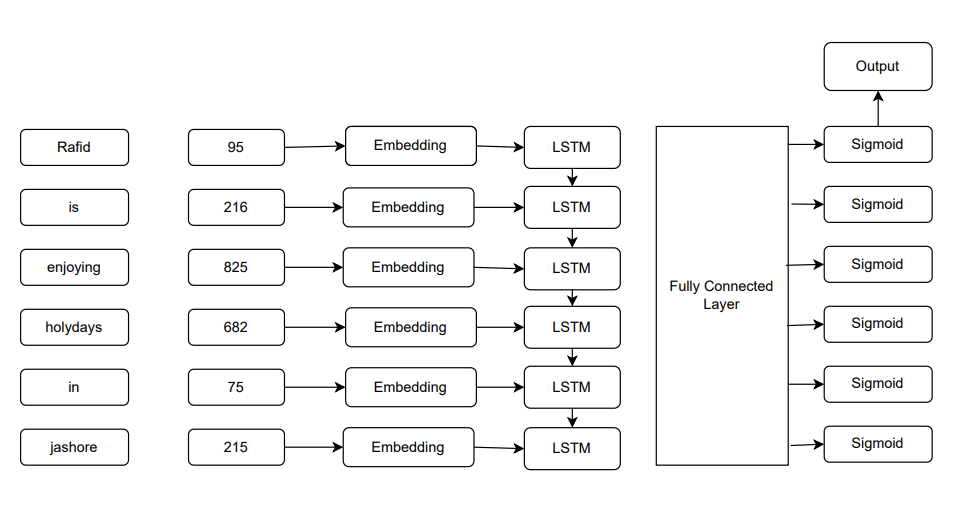
\includegraphics[width=\linewidth]{chapters/LSTM.png}
  \caption{LSTM architecture}
\end{figure}

There are mainly five layers in LSTM network. But layer an be added to improve the accuracy of the model. The five layers are:
\begin{itemize}
\item \textbf{Embedding Layer:} This Layer is responsible for converting word tokens into embedding of a specific size like 256, 512 etc. This layer maps a sequence of word indices to embedding vectors and learns the word embedding during training.
In this layer the word tokens are converted into embedding of a specific size like 256,512 etc. This layer also responsible for mapping a sequence of word indices to embedding vectors and learns the word embedding during training.

\item \textbf{LSTM Layer:}This layer sequentially process data and keep its hidden state through time. It keeps previous memory and process with current memory and decides whether to keep current memory or remain with old memory.
   
\item \textbf{Fully Connected Layer:} This layer indicates those layers where all inputs from one layer are connected to every unit of the next layer.

\item \textbf{Sigmoid Activation Layer:} This layer is responsible for converting all output values in the range of 0 to 1. It means it can either let no flow or complete flow of information throughout the gates.

\item \textbf{Output Layer:} Output layer is the final layer of the architecture. This layer is responsible for generating output which is obtained from sigmoid layer. The output formate is 2d array of real numbers where the first dimension indicates the number of samples given to the LSTM layer and second dimension is the dimensionality of the output space defined by the units
parameter in Keras LSTM implementation.
\end{itemize}


% Chapter-4
\chapter{Implementation} \label{ch:implementation}
Theoretically everything works on paper but a method can not be justified completely unless it is implemented and tested as well. This chapter emphasizes on requirements for running the model and how the model is actually built and its working principle.

\section{System Requirements}
Deep learning models often require heavy hardware to operate faster. These models can be run on lower end desktop computers but training the data and testing it would take a lot of time. There are two methods of working on these models
\begin{itemize}
\item Using PAAS Services namely Google Colab
\item Using Jupyter Notebook on local machine
\end{itemize} 
\subsection{Using PAAS Services}
Platform as a service or simply PAAS provides necessary hardware and software support for development purposes based on subscription or fees. For our model, Google Colab is a great service that provides great support to a certain range for free of cost. It is a hosted jupyter notebook service that requires no setup to use while providing resources to build models for example gpus~\cite{url1}. Only requirement in this case is a stable internet connection and a functioning computer device with a browser.
\subsection{Using Jupyter Notebook}
Jupyter notebook is a web-based interactive computational environment which is used by wide variety of developers for managing and integrating big data tools~\cite{url2}. In order to use it on local machine, one will need certain hardware capabilities to work with machine learning models.
\begin{table}
\centering
\begin{tabular}{|l|l|}
\hline
Type & Specification \\
\hline
CPU & Any Quad core CPU with at least 2.1 GHZ base speed \\
\hline
Ram & 8 gigabytes \\
\hline
GPU(Optional) & 8 gigabytes of vram or higher for faster computation \\
\hline
OS & Linux, Windows, MacOS \\
\hline
\end{tabular}
\caption{Hardware and OS Requirement for Jupyter Notebook}
\end{table}


\section{Dataset}
Dataset for the proposed emotion detection model contains 16000 thousand lines of dialogue for training purposes, 2000 lines of dialogue each for validation and testing purposes. Pandas was used here for data analysis and data manipulation. Pandas is a powerful and easy to use open source software library which is used for data analysis and manipulation. It offers data structures and operations for manipulating numeric tables and time series~\cite{ref11}.

\section{Preprocessing}
Dataset used for the proposed model is mainly text based and only contained plain anonymous messages. However, the dialogues or messages contained coma signs, full stop signs and a lot of the letters are in upper case or lower case form. Using python libraries, these anomalies are normalized. For further preprocessing, label encoding, a python library is used which is a technique for converting categorical columns into numerical columns so they can be fitted by models. It is an important preprocessing step.~\cite{url3} 

\section{Use of Tokenization}
There are thousands of words in the used dataset and there are words that were used multiple times in different sentences. By using tokenizer which is a library function of keras, it was possible to turn texts into tokens which is later indexed or vectorized~\cite{url4}. Here, the words are indexed based on the frequency of occurrences.
\section{Glove Embedding}
Glove wiki gigaword 300 was used as glove embedding. Glove embedding basically helps in catching similar words in dataset and make vector representations of those words. It is an unsupervised learning algorithm~\cite{url5}.
\section{Model Building}
The proposed model is mainly using LSTM to make predictions on emotion on given dataset. For training the model, training dataset was used with validation dataset to improve accuracy. Here lower batch size is considered for better feature extraction. Moreover, there are eight layers in the proposed model. The layers are as follows-
\begin{itemize}
\item Embedding Layer
\item LSTM Layer
\item 3 Dropout Layers
\item 2 Dense Layers with sigmoid activation function
\item Activation Layer with softmax function
\end{itemize}
\subsection{Embedding Layer}
Embedding layer is a type of hidden layer which maps input information from high dimensional to a lower dimensional space. For this model, the embedding class from keras API was used. The vocabulary size of dataset was used as input dimension and output dimension was used similar to glove embedding's dictionary dimension size which uses 300 length vectors to represent each word.
\subsection{LSTM Layer}
Keras API provides a great way to implement lstm layer with customizable parameters. The proposed model used lstm layer with 256 memory units that represent the dimensionality of outer space. This layer will classify and make predictions on the time series data.
\subsection{Dropout Layers}
The proposed model utilizes multiple dropout layers to tackle overfitting. In case of overfitting, the model is designed to drop 25\% of nodes in the neural network training processes and act as if they are not part of the network architecture. 
\subsection{Dense Layers}
Dense layers acts as a layer in which neurons receive input from all the previous layers. The proposed model includes two dense layers. One of the dense layers has a activation function named sigmoid and consists of 64 neural units. The second dense layer includes only six neural units
\subsection{Activation Layer}
Softmax activation function is used in the proposed model. It converts vector of values to probability distribution where the output vector are in range from 0 to 1. Here the softmax function is used for the last layer of emotion classification network because the result is to be interpreted as a probability distribution.

\subsection{Use of Optimizer and EarlyStopping}
For further improving the model, Adam optimizer is used with a learning rate of 0.0005 which greatly improves learning capacity of network. In order to further avoid unnecessary training cycles, early stopping is implemented with patience set to nine. Therefore if the network doesn't face improvements over nine epochs, it will stop training process of the model.


% Chapter-5
\chapter{Testing and Result Analysis}
This chapter emphasizes the testing and result analysis procedure of our model. Testing and result analysis are vital component of the development and assessment process for any model. Testing is a systematic procedure of evaluating a model's performance based on various measures. Where the goal is to ensure that the model meets it's expected requirements. On the other hand the result analysis involves analysing the outcome of the testing process. This process interprets  model's performance and effectiveness in various metrics and calculations.

\section{Testing Procedure}
About four thousands of text data are used to test the performance of our built model. Where two thousands are used as validation data and another two thousands are used as test data. Here totally different text data are used for finding out the actual performance of our model.

\section{Model Evaluation}
Model evaluation is a process which help us to measure the performance of a model based on some metrics. This procedure in needed for a model to check whether the model meets the expected performance or not. This also helps to find out the weakness of a model. There are many types of metrics for evaluating a model. Such as Accuracy, Precision, Recall , F1 score etc. This section emphasizes some of the performance measure metrics which are used to evaluate the performance of our model.
\subsection{Confusion Matrix}
Most of the performance metrics are measured based on the confusion matrix. It's a two dimensional table which consists of actual value and predicted value. And four types of value are represented in this table based on these two types of value. Which are True Positive(TP), False Positive(FP), False Negative(FN) and True Negative(TN). True positive and true negative represents the term when actual value and predicted value are same. Where false positive and false negative represents the mismatch between actual value and predicted value.

\begin{table}[h!]
\centering
\begin{tabular}{|l|l|l|}
\hline
& Actual Positive (1) & Actual Negative (0)\\
\hline
Predicted Positive (1) & True Positive (TP) & False Positive (FP)  \\
\hline
Predicted Negative (0) & False negative(FN) & True Positive(TP) \\
\hline
\end{tabular}
\caption{Confusion Matrix}
\end{table}

\subsection{Accuracy}
Accuracy represents the model's correct predictions in a mathematical form. It defines how close the prediction to the actual value.
The formula for calculating accuracy is,
\begin{equation}
Accuracy = {\frac{TP+TN}{TP+TN+FP+FN}}
\end{equation}

\subsection{Precision}
Precision represents how close the measure value to each other. Here the value of true positives are divided by the total predicted positives,
\begin{equation}
Precision = {\frac{TP}{TP+FP}}
\end{equation}

\subsection{Recall}
Recall defines the ratio of all correctly predicted positive predictions. Here the value of true positive predictions are divided by all positive predictions.
\begin{equation}
Recall = {\frac{TP}{TP+FN}}
\end{equation}

\subsection{F1 Score}
F1 score represents the overall test accuracy of a model. It provides feedback based on precision and recall.
\begin{equation}
F1 Score = {\frac{2*(Precision*Recall)}{Precision+Recall}}
\end{equation}

\section{Results And Discussion}
We use a data-set for the implementation of our LSTM architecture is mainly text based contained total 20000 thousand plain anonymous messages. We investigated our architecture in two ways. First we ran the model without using Word Embedding, then we found improvements in training, testing and validation accuracy using GloVe Embedding. LSTM architecture gives 0.8245 as Testing Accuracy without using Embedding while using Embedding the architecture gives 0.9255. Also, we have greatly reduced training and validation losses by using GloVe. The proposed model is trained with a limit of 70 epochs.

\begin{table}[h!]
\centering
\begin{tabular}{|c|cc|cc|cc|}
\hline
\multirow{2}{*}{Model} & \multicolumn{2}{c|}{Training}         & \multicolumn{2}{c|}{Validation}       & \multicolumn{2}{c|}{Testing}          \\ \cline{2-7} 
                       & \multicolumn{1}{c|}{Accuracy} & Loss  & \multicolumn{1}{c|}{Accuracy} & Loss  & \multicolumn{1}{c|}{Accuracy} & Loss  \\ \hline
LSTM Without GloVe     & \multicolumn{1}{c|}{92.1\%}   & 1.9\% & \multicolumn{1}{c|}{83.2\%}   & 4.2\% & \multicolumn{1}{c|}{82.45\%}  & 4.5\% \\ \hline
LSTM With GloVe        & \multicolumn{1}{c|}{97.8\%}   & 0.5\% & \multicolumn{1}{c|}{93.1\%}   & 1.7\% & \multicolumn{1}{c|}{92.55\%}  & 1.8\% \\ \hline
\end{tabular}
\caption{Model Accuracy Comparison}
\end{table}

Table 5.2. The table shows the model accuracy comparison while using and not using GloVe with the model. So, to get better results using Word Embedding with LSTM found more effective.

We have worked with 6 emotions in our model. Precision, recall, F1-scores for different emotions are shown in Table 5.3.


\pagebreak

\begin{table}[h!]
\centering
\begin{tabular}{|c|c|c|c|}
\hline
Emotion       & Precision & Recall & F1-Score \\ \hline
Sadness       & 0.92      & 0.94   & 0.93     \\ \hline
Anger         & 0.88      & 0.90   & 0.89     \\ \hline
Love          & 0.92      & 0.96   & 0.94     \\ \hline
Surprise      & 0.91      & 0.77   & 0.84     \\ \hline
Fear          & 0.97      & 0.96   & 0.96     \\ \hline
Joy           & 0.79      & 0.73   & 0.76     \\ \hline
Accuracy      & -         & -      & 0.93     \\ \hline
Marco Avg.    & 0.90      & 0.88   & 0.89     \\ \hline
Weighted Avg. & 0.93      & 0.93   & 0.92     \\ \hline
\end{tabular}
\caption{The results obtained for Six Emotions}
\end{table}

Table 5.3. The Table shows among the 6 emotions,  the F1-Score of 'Fear' is the highest, the scores of other emotions are also close. F1-score's accuracy 0.93. F1-score's macro avg. and weighted avg. 0.89 and 0.92.

% Chapter-6
\chapter{Conclusions}\label{ch:conclusion}

\section{Conclusions}


\section{Future Prospects of Our Work}



% Chapter showing example of index creation
%\chapter{Index Creation}
\section{BUET}
Bangladesh University of Engineering and Technology, abbreviated as
BUET\index{BUET}, is one of the most prestigious institutions for
higher studies in the country. About 5500 students are pursuing
undergraduate\index{BUET!undergraduate} and
postgraduate\index{BUET!postgraduate} studies in engineering,
architecture, planning and science in this institution. At present,
BUET has sixteen teaching departments under five faculties and it has
three institutes. Every year the intake of undergraduate students is
around 900, while the intake of graduate students in Master's and PhD
programs is around 1000. A total of about five hundred teachers are
teaching in these departments and institutes. There are additional
teaching posts like Dr.\ Rashid Professor, Professor Emeritus and
Supernumerary Professors.
 
\section{Campus}
The BUET campus is in the heart of Dhaka\index{Dhaka} --- the capital
city of Bangladesh. It has a compact campus with halls of residence
within walking distances of the academic buildings. The physical
expansion of the University over the last three decades has been
impressive with construction of new academic buildings,
auditorium\index{BUET!auditorium} complex, halls of residence, etc.
 
\section{History}\index{BUET!History}
BUET is the oldest institution for the study of Engineering and
Architecture in Bangladesh. The history of this institution dates back
to the days of Dhaka Survey School which was established at
Nalgola\index{Nalgola}, in Old Dhaka in 1876 to train Surveyors for
the then Government of Bengal of British India. As the years passed,
the Survey School became the Ahsanullah School of
Engineering\index{Ahsanullah School of Engineering} offering
three-year diploma courses in Civil, Electrical and Mechanical
Engineering. In recognition of the generous financial contribution
from the then Nawab of Dhaka, it was named after his father Khawja
Ahsanullah. It moved to its present premises in 1912. In 1947, the
School was upgraded to Ahsanullah Engineering College as a Faculty of
Engineering under the University of Dhaka, offering four-year
bachelor’s courses in Civil, Electrical, Mechanical, Chemical and
Metallurgical Engineering. In order to create facilities for
postgraduate studies and research, Ahsanullah Engineering College was
upgraded to the status of a University in 1962 and was named East
Pakistan University of Engineering and Technology. After the War of
Liberation in 1971\index{1971|see {War of Liberation}}\index{War of
  Liberation}, Bangladesh became an independent state and the
university was renamed as the Bangladesh University of Engineering and
Technology.
 
\section{Students}
Till today, it has produced around 25,000 graduates in different
branches of engineering and architecture, and has established a good
reputation all over the world for the quality of its graduates, many
of whom have excelled in their profession in different parts of the
globe. It was able to attract students from countries like
India\index{India}, Nepal\index{Nepal}, Iran\index{Iran},
Jordan\index{Jordan}, Malaysia\index{Malaysia}, Sri Lanka\index{Sri
  Lanka}, Pakistan\index{Pakistan} and Palestine\index{Palestine}.
 
\section{Departments}
Both Undergraduate and Postgraduate studies and research are now among
the primary functions of the University. Eleven departments under five
faculties offer Bachelor Degrees, while most of the departments and
institutes offer Master's Degrees and some of the departments have
Ph.D. programs. In addition to its own research programs, the
university undertakes research programs sponsored by outside
organizations like European Union, UNO,
Commonwealth\index{Commonwealth}, UGC\index{UGC}, etc. The expertise
of the University teachers and the laboratory facilities of the
University are also utilized to solve problems and to provide
up-to-date engineering and technological knowledge to the various
organizations of the country.


\endinput


% Bibliographies and appendices
	
\renewcommand{\bibname}{References}
\begin{thebibliography}{8}
\bibitem{ref1}
Wang X, Kou L, Sugumaran V, Luo X, Zhang H. Emotion correlation mining through deep learning models on natural language text. IEEE transactions on cybernetics. 2020 May 13;51(9):4400-13.

\bibitem{ref2}
Fei H, Ji D, Zhang Y, Ren Y. Topic-enhanced capsule network for multi-label emotion classification. IEEE/ACM Transactions on Audio, Speech, and Language Processing. 2020 Jun 10;28:1839-48.

\bibitem{ref3}
Krommyda M, Rigos A, Bouklas K, Amditis A. An experimental analysis of data annotation methodologies for emotion detection in short text posted on social media. InInformatics 2021 Mar 12 (Vol. 8, No. 1, p. 19). MDPI.

\bibitem{ref4}
Chiorrini A, Diamantini C, Mircoli A, Potena D. Emotion and sentiment analysis of tweets using BERT. InEDBT/ICDT Workshops 2021 Mar 23 (Vol. 3).

\bibitem{ref5}
Pepino L, Riera P, Ferrer L, Gravano A. Fusion approaches for emotion recognition from speech using acoustic and text-based features. InICASSP 2020-2020 IEEE International Conference on Acoustics, Speech and Signal Processing (ICASSP) 2020 May 4 (pp. 6484-6488). IEEE.

\bibitem{ref6}
Yang X, Feng S, Zhang Y, Wang D. Multimodal sentiment detection based on multi-channel graph neural networks. InProceedings of the 59th Annual Meeting of the Association for Computational Linguistics and the 11th International Joint Conference on Natural Language Processing (Volume 1: Long Papers) 2021 Aug (pp. 328-339).

\bibitem{ref7}
Graterol W, Diaz-Amado J, Cardinale Y, Dongo I, Lopes-Silva E, Santos-Libarino C. Emotion detection for social robots based on NLP transformers and an emotion ontology. Sensors. 2021 Feb 13;21(4):1322.

\bibitem{ref8}
Sharma T, Diwakar M, Singh P, Lamba S, Kumar P, Joshi K. Emotion Analysis for predicting the emotion labels using Machine Learning approaches. In2021 IEEE 8th Uttar Pradesh Section International Conference on Electrical, Electronics and Computer Engineering (UPCON) 2021 Nov 11 (pp. 1-6). IEEE.

\bibitem{ref9}
Yu Y, Si X, Hu C, Zhang J. A review of recurrent neural networks: LSTM cells and network architectures. Neural computation. 2019 Jul 1;31(7):1235-70.

\bibitem{ref10}
Mohammed SM, Jacksi K, Zeebaree SR. Glove word embedding and DBSCAN algorithms for semantic document clustering. In2020 International Conference on Advanced Science and Engineering (ICOASE) 2020 Dec 23 (pp. 1-6). IEEE.

\bibitem{url1}
Colab, \url{https://colab.google/}. Last Accessed December 1, 2023

\bibitem{url2}
Project Jupyter, \url{https://en.wikipedia.org/wiki/Project_Jupyter}. Last Accessed December 1, 2023

\end{thebibliography}

% Index, comment this out if you do not want to create an index
\printindex

\appendix
% Algorithms
%\input{chapters/algorithms.tex}

\end{document}